\chapter{Intended research directions}
\label{chap:future}

In this chapter, we outline the proposed future research directions and ideas. The main focus is \todo{Fill in afterwards}.

\todo[inline]{Chapter outline}

\section{Applications in cybersecurity}

Cybersecurity is an ever-evolving field, constantly challenged by sophisticated attacks and the increasing complexity of digital infrastructures. As cyber threats grow more advanced, traditional security measures often fall short in detecting and mitigating these evolving threats. Graphs are a natural representation for many cybersecurity applications. For example, computer networks, social networks, and software codebases can all be modeled as graphs where nodes represent entities (such as devices, users, or functions) and edges represent the relationships or interactions between these entities. This representation enables a holistic view of the complex and interconnected nature of cybersecurity environments. By utilizing graph models, cybersecurity practitioners can analyze the interdependencies and patterns of behavior across entire networks, allowing for more effective threat detection and response.

Graph Neural Networks (GNNs) extend the power of traditional graph-based models by incorporating deep learning techniques. Unlike conventional neural networks, GNNs are designed to operate directly on graphs, capturing both the features of individual nodes and the structural information of the graph as a whole. This capability makes GNNs particularly well-suited for cybersecurity tasks, such as identifying anomalous patterns in network traffic, detecting malware in executable files, or uncovering hidden relationships in social engineering attacks. By learning from the complex, high-dimensional data that typifies cybersecurity challenges, GNNs provide a robust approach to understanding and counteracting cyber threats.

The application of graph machine learning to cybersecurity has been the primary motivation behind our research in the past as continues to be the main source of problems and ideas into the future. To underscore this, let us consider the research presented in Chapter~\ref{chap:my-research} -- The performance-complexity framework and both of the subsequent graph coarsening techniques were originally conceived to solve the problem of too large graphs in network traffic analysis, where a simple graph of network connections may have on the order of millions of nodes. Similarly, studying the effect graph properties have on downstream tasks (as presented in Section~\ref{sec:graph-property-effect}) is motivated by the problem of constructing a graph from data in such a way that the graph is both representative of the problem being solved and has advantageous properties for GNN processing. This is again a problem closely related to network traffic analysis, where large amounts of data are collected and the correct way of filtering them and constructing a graph from them is an open problem.\todo{If we add CSP, mention it here as well}

\todo[inline]{Maybe introduce the particular problems we are solving? Along the lines of the "GNN-Based Malicious Network Entities Identification In Large-Scale Network Data" paper}

Continuing into the future, this application domain remains of high interest to us. As shown by the previously conducted research, the problems arising from applying general machine learning models to a specific domain usually aren't limited to that singular domain or may be specific cases of obstacles to applying the methods more generally. Thus, although we seek to research algorithms and approaches that generalize across application domain, the choice of a specific domain as the intended usage of those approaches serves as a good guide to discovering relevant problems and interesting research opportunities.

\section{Explainable graph models}

Despite the relatively high performance of GNNs in identifying cyber threats among other applications, these models essentially operate as "black boxes," making their decision-making processes difficult to understand. This lack of transparency poses significant challenges particularly in cybersecurity, where understanding the rationale behind model predictions is crucial. Graph explainability -- the ability to interpret and explain the outputs of graph-based models—thus becomes essential in ensuring these tools are both effective and trustworthy.

In cybersecurity, the stakes are high. Decisions made by machine learning models can have far-reaching consequences, such as determining whether a network anomaly is benign or indicative of a sophisticated attack. Without clear explanations, security analysts might find it difficult to trust the model's predictions, leading to skepticism or hesitation in acting upon the model's recommendations. Explainable graph models help bridge this gap by providing insights into why certain patterns were flagged as malicious or why particular nodes (representing devices, users, or files) were identified as potential threats. This transparency not only increases trust in automated systems but also aids analysts in making more informed decisions.

Graph explainability also plays a critical role in improving the models themselves. By understanding why a model makes certain predictions, cybersecurity professionals can identify biases, correct inaccuracies, and refine algorithms to better detect evolving threats. For example, if a model consistently fails to recognize a particular type of attack, explainability tools can help pinpoint where the model's reasoning is flawed, allowing for targeted improvements. This iterative process is essential for keeping pace with the constantly evolving nature of cyber threats.

In our research, there are several open questions we would like to explore in the future, which are listed in the rest of this section.

\subsubsection{Which explanation algorithm is the most suitable for the domain?}

When comparing GNN explainer algorithms for application in cybersecurity, it's crucial to consider the specific needs of the domain, such as the interpretability of complex, interconnected data and the ability to detect subtle patterns indicative of malicious activities. Algorithms like GNNExplainer and PGExplainer offer node-level and edge-level explanations by identifying the most relevant subgraphs or node features that contribute to a prediction, which can be particularly useful in cybersecurity for explaining why a specific alert was raised. On the other hand, algorithms like SubgraphX\todo{Not described in the theoretical part} focus on identifying critical subgraphs that influence model predictions, making them ideal for understanding larger patterns, such as the spread of a phishing campaign across a network. Model-agnostic methods like GraphLIME provide flexibility by offering explanations that are not tied to a specific GNN architecture, which is advantageous when dealing with diverse datasets and threat scenarios. In our application, the explanations target both skilled security analysts as well as ordinary network administrators, adding yet another dimension of the complexity of the explanation and its use-cases, where network administrators are usually interested in specific threats in the network, while security analysts might take a broader view and want to move laterally to uncover the whole threat across the dataset.

\subsubsection{How to deal with hypergraphs?}

Applying graph explainers to hypergraphs presents unique challenges due to the complexity of the relationships they represent. Unlike traditional graphs, where edges connect pairs of nodes, hypergraphs involve hyperedges that can connect multiple nodes simultaneously, creating a higher-order structure that captures more complex interactions. This increased complexity makes it difficult to develop graph explainer methods that can effectively handle the multidimensional nature of hypergraphs. Additionally, hypergraphs by definition involve overlapping communities and non-pairwise relationships, which are not easily captured by standard graph metrics or traditional machine learning models. As a result, designing explainers for hypergraphs requires new approaches to interpret the interactions within hyperedges and the overall structure of the graph. Furthermore, the lack of standard benchmarks and evaluation metrics for hypergraph explainability adds to the difficulty of assessing the quality and relevance of explanations, making it challenging to develop robust and interpretable models that can provide insights into hypergraph data.

In our use-case, hypergraphs are a common structure for representing relationships between different computer network entities. Every hypergraph \( H = \left( V, E \right) \) corresponds to a bipartite \name{incidence graph}, also called the Levi graph (see \cite{levi_finite_1942}). This bipartite graph \( G= \left( V \cup E, E_\mathrm{bip} \right) \) has as its two partitions the nodes and hyperedges of \( H \), and its edges represent a node in \( V \) belonging to an edge in \( E \), formally \( E_\mathrm{bip} = \left\{ \left( v_i, e_j \right) \in V \times E \middle| v_i \in e_j \right\} \). This duality between hypergraphs and bipartite graphs is useful when describing e.g.\ relationships between different computer network entities. When studying connection of different users to a set of server, one can look at this as a bipartite graph with the users and servers being the two partitions. At the same time, when only relationships between users are of interest, the hypergraph representation where servers form hyperedges between users may be more intuitive and useful.

Existing graph machine learning algorithms and graph explainers struggle with bipartite graph. As presented in Section~\ref{sec:graph-property-effect}, graph homophily (the tendency of nodes of the same class to cluster together) is the most indicative property for GNN performance. Bipartite graph fundamentally break this assumption as every edge connects two dissimilar nodes. While there are some preliminary works towards the resolution of this issue (see \cite{maleki_learning_2023}), the subject is not sufficiently studied and warrants further research.

\subsubsection{How to combine multiple modalities in one explanation?}

Graph Neural Networks (GNNs) have shown tremendous potential in analyzing and learning from multi-modal graphs, which are graphs that integrate multiple types of nodes, edges, and features from diverse data sources. In cybersecurity, multi-modal graphs can represent complex relationships between various entities such as users, devices, network connections, and threat indicators, each contributing different types of information. GNNs are particularly well-suited for this setting as they can learn to propagate and aggregate information across heterogeneous nodes and edges, capturing the intricate dependencies and interactions present in multi-modal data. By leveraging the rich contextual information embedded within multi-modal graphs, GNNs can enhance the detection of sophisticated cyber threats, uncover hidden patterns, and provide deeper insights into the nature of cyber attacks. This ability to model and interpret complex, multi-source data makes GNNs a powerful tool for developing more robust and effective cybersecurity solutions.

On the other hand, the issue of explaining GNN predictions on multi-modal graphs is not well studied. In our preliminary work, we have tried several approaches to tackling multi-modal graphs from treating them as separate graphs with the same nodes and differing edges, treating connections of different modalities as separate edges in the same graph, allowing for multiple edges between 2 nodes or merging edges of different modalities into one and adding modality flags as edge features -- which so far seems to be the most promising approach. However, a more thorough exploration of the interplay between modalities and explanations is needed, as for example explanations using edge masks may need to treat the different modalities separately.

\subsubsection{How to filter large graphs, while keeping the explanations relevant?}

As outlined in our previous works described in Section~\ref{sec:performance-complexity}, large graphs pose an obstacle to traditional graph machine learning models. Applying graph explainers to very large graphs also presents significant challenges due to the scale and complexity of the data involved. Graph explainers typically require the exploration of subgraph structures and the evaluation of numerous potential explanations, which can become prohibitively expensive in terms of time and computational resources when dealing with vast graphs. Additionally, the interpretability of explanations diminishes as the size of the graph grows, making it harder to identify meaningful patterns or insights amidst the vast amount of information. Furthermore, the inherent noise and redundancy in large graphs can lead to explanations that are either too broad to be useful or too specific to generalize well.

To overcome these obstacles, the development of more efficient and scalable graph explainer methods could be undertaken. Such an approach, however, ight not be necessary and may be overcomplicated. Instead, we are examining a pre-processing of the graph that would decrease its complexity. We have so far examined using simple graph tools like filtering according to the \name{Rich-club coefficient} (see \cite{zhou_rich-club_2004}). Furthermore, our previous works on graph coarsening described in Sections~\ref{sec:harp-coarsening} and~\ref{sec:direct-coarsening} may be applicable to the problem of producing reasonably sized explanations as well. Finally, our previous study of graph properties and their effect on GNN performance, presented in Section~\ref{sec:graph-property-effect} may give us a framework for easy evaluation of the effectiveness of any applied pre-processing.

\section{GNN hyper-parameter optimization guided by graph properties}
\label{sec:gnn-hpo}

A second area of intended future research is in the field of hyper-parameter optimisation for graph neural networks. In Section~\ref{sec:graph-property-effect}, we presented our work studying the effect of graph properties on downstream classifier performance. As part of \cite{prochazka_which_2023}, we also carried out a preliminary study of the interplay between graph properties, model hyper-parameters and GNN performance. For each dataset used (of which there were 139 when counting each binary classification problem separately), 108 unique hyper-parameter configurations were considered and a GraphSAGE model was trained with them. This gave us a meta-dataset of 15 012 different combinations of graph properties, hyper-parameter values and associated GNN performance metrics. This meta-dataset was subsequently used to train a meta-model predicting GNN performance from the graph properties and hyper-parameter values. As the meta-model, we used a random forest regression model -- the choice of a simple model was sufficient to achieve good predictive power and at the same time evaluating the meta-model is so computationally cheap when compared to the GNN that it is possible to carry out a total exploration of the hyper-parameter configuration space using the meta-model.

\begin{figure}
	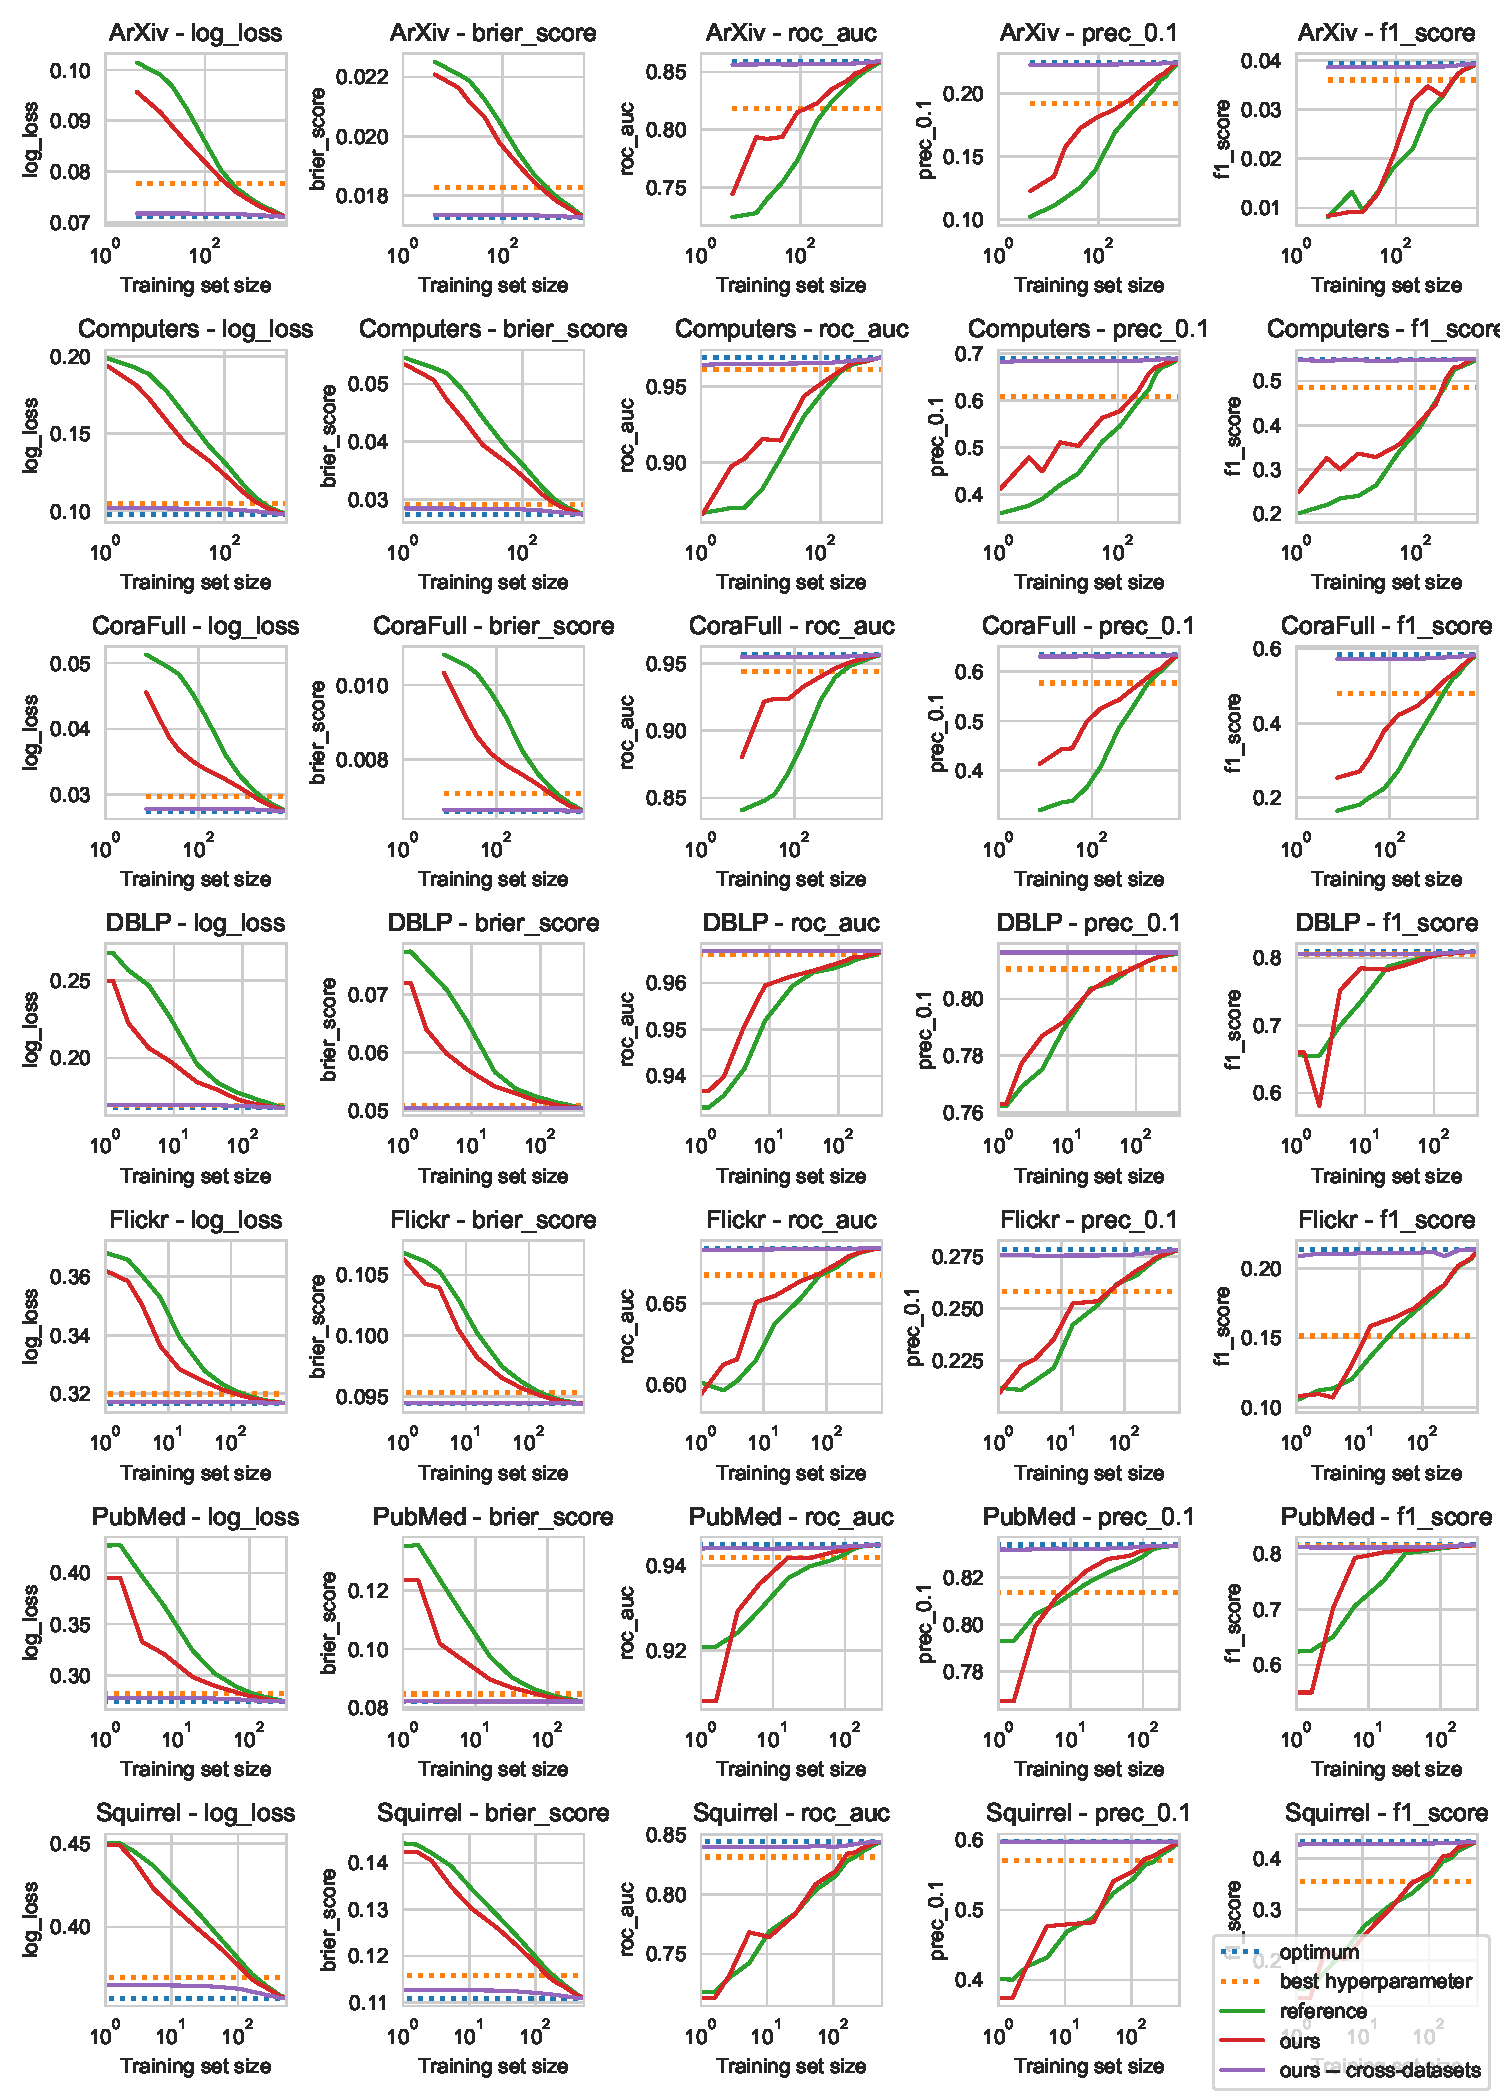
\includegraphics[width=\linewidth]{images/gnn-hpo.pdf}
	\caption{Comparison of reference random hyper-parameter search with the proposed solutions for considered datasets. While log-loss and Brier score (two columns from left) are to be minimised, the remaining performance metrics are to be maximised. We stress that the violet curve is very close to the (optimal) blue dotted line for almost all datasets and target metrics. It means that the proposed way of hyper-parameter tuning is able to reveal almost optimal hyper-parameter setup based only on the actual graph properties. Original figure from \cite{prochazka_which_2023}.}
	\label{fig:gnn-hpo}
\end{figure}

Figure~\ref{fig:gnn-hpo} shows the results of this experimental setup. We compared our approach to reference random search strategy for hyperparameter optimization. The evaluation compares the best performance value obtained by each hyperparameter optimization strategy as a function of number of evaluations of the GNN model (which corresponds to the training set size of the meta-model). The proposed meta-model-based approach was used in two different fashions. In the first approach, the meta-model was trained only on GNN runs for the currently evaluated dataset. This approach (red line in the plot) approached the performance optimum faster or roughly as quickly as random search. Secondly, the cross-dataset approach used a meta-model that was pre-trained on GNN runs on other datasets, excluding the currently evaluated dataset. This approach (violet line in the plot) reached near-optimal performance without needing even one run of the GNN on the evaluated dataset.

The results of the cross-dataset hyperparameter optimization strategy are extraordinary in that they point to a possible \enquote{zero-shot} optimization strategy from GNNs - i.e.\ a strategy that produces competitive hyperparameter configurations for a given graph dataset without needing to run the GNN even once. These results, however, need further verification and development. Our paper \cite{prochazka_which_2023} is mainly concerned with the effect of graph properties on GNN performance and hyperparameter optimization is only an auxiliary result. We intend to carry out a full and thorough study of this effect in the future.
